\documentclass{article}

\usepackage[most]{tcolorbox}
\usepackage{physics}
\usepackage{graphicx}
\usepackage{float}
\usepackage{amsmath}
\usepackage{amssymb}


\usepackage[utf8]{inputenc}
\usepackage[a4paper, margin=1in]{geometry} % Controla los márgenes
\usepackage{titling}

\title{Clase 8}
\author{Manuel Garcia.}
\date{\today}

\renewcommand{\maketitlehooka}{%
  \centering
  \vspace*{0.05cm} % Espacio vertical antes del título
}

\renewcommand{\maketitlehookd}{%
  \vspace*{2cm} % Espacio vertical después de la fecha
}

\newcommand{\caja}[3]{%
  \begin{tcolorbox}[colback=#1!5!white,colframe=#1!25!black,title=#2]
    #3
  \end{tcolorbox}%
}

\begin{document}
\maketitle

\section{Cauchy }
\caja{green}{Definición }{
  una secuencia $ \{a_n \}_{n= 1 } ^ {\infty} $, se llama cauchy si para cada $ \epsilon >0  $, hay un entero $ N  $ tal que: 
  \begin{gather*}
    \left|a_n - a_m \right|<\epsilon \quad \text{Para todo }m,n \geq N
  \end{gather*}
}
\caja{green}{Teorema }{
  Una secuencia d enúmeros complejos $ \{a_n \}_{n=1 } ^ {\infty} $ converge si y solo si es una secuencia de cauchy.
}
\textbf{Demostracion } Supongamos que $ \{a_n \}_{n=1 } ^ {\infty} $ converge a $ L  $. Dado $ \epsilon>0  $, y $ N  $, tal que $ m,n \geq N  $. Esto implica que $ \left|a_n - L \right|<\frac{\epsilon}{2} $ y $ \left|L-a_m \right|<\frac{\epsilon}{2} $

\begin{gather*}
  \left|a_n - L + L - a_m \right| < \left|a_n -l \right|+ \left|L-a_m \right|<\epsilon\\
  \left|a_n - a_m \right|< \epsilon\\
  \text{\textbf{"Si la secuencia converge es una secuencia de Cauchy"}}
\end{gather*}

Y si es en la otra direccion? 
El reciproco lo demostramos partiendo de que la secuencia $ \{a_n \} _{n=1 } ^ {\infty} $ es una secuencia de Cauchy. Entonces, dado $ \epsilon>0  $ existe $ N  $ tal que $ \left|a_n - a_m \right|<\epsilon $ para todo $ n,m \geq N  $.

Si escribimos $ a_n = x_n + i y_n  $ y $ a_m  = x_m + i y_m  $ con $ x_n,x_m,y_n,y_m \in \mathbb{R} $. Recordemos que en todo complejo se satisface que: $ \left|Re(z )\right|\leq \left|z \right|, \quad \left|Im(z) \right|\leq \left|z \right| $.

Entonces $ \left|x_n - x_m\right| \leq \left|a_n - a_m \right| $, $ \left|y_n - y_m \right|\leq \left|a_n - a_m \right| $
\begin{gather*}
  \left|x_n - x_m \right|<\epsilon, \qquad \left|y_n - y_m \right|<\epsilon\\
  \text{La secuencia }\{a_n \}_{n=1 } ^ {\infty} \text{ converge}\\
  \text{\textbf{"Si es de Cauchy entonces la secuencia converge"}}
\end{gather*}
\begin{figure}[H]
  \begin{center}
    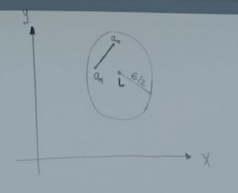
\includegraphics[width=0.4\textwidth]{cauchy.png}
  \end{center}
\end{figure}


\section{Series }
\begin{gather*}
  \sum_{n= 0 }^{\infty} a_n = a_0 + a_1 + a_2 + ... + a_n + ...\\
  S_n = \sum_{n= 0 }^{N }a_n = a_0 + a_1 + a_2 + ... + a_n + ... 
\end{gather*}
La serie converge si $ \underset{N \rightarrow \infty}{lim }S_n = S  $ con $ S \in \mathbb{C} $. 

\textbf{Ejemplo } Muestre que si $ \left|z \right|< 1  $ entonces la serie geométrica $ \sum_{n= 0 }^{\infty} z ^ {n } $ converge a $ \frac{1}{1-z } $ y por lo tanto $ \sum_{n=0 }^{\infty}z ^ {n } =  \frac{1}{1-z } $ y diverge para cualquier otro caso. 
\begin{gather*}
  S_N = 1 + z+z ^ {2 } + ... + z ^ {N }\\
  z S_N = z + z ^2 + z ^ {3 }+ ... + z ^ {N + 1 }\\
  1 + z S_N = 1 + z + z ^2 + ... + z ^ {N + 1 }\\
  1 + z S_N = S_n + z ^ {N+1 }\\
  S_N (1 - z) = 1-z ^ {N+ 1 } \quad \rightarrow \quad S_N = \frac{1- z ^ {N+ 1 }}{1 - z }\\
  \underset{N \rightarrow \infty}{lim } S_N = \underset{N \rightarrow \infty}{lim }\frac{1 - z ^ {N+1 }}{1 - z } = \frac{1}{1-z}
\end{gather*}
Conclusion: $ \sum_{n= 0 }^{\infty}z ^ {n } = \frac{1}{1-z }, \quad \left|z \right|<1$.

\caja{blue}{Ejercicio }{
  Discutir la convergencia de la serie: 
  \begin{gather*}
    \displaystyle\sum_{n= 0 }^{\infty}\frac{1}{(6 + 8z )^ {n }}
  \end{gather*}
}
\textbf{Solucion }
\begin{gather*}
  \displaystyle\sum_{n= 0 }^{\infty}\frac{1}{(6 + 8z )^ {n }} = \displaystyle\sum_{n= 0 }^{\infty}\left[\frac{1}{(6 + 8z )}\right]^ {n }\\
  \left|\frac{1}{6+ 8z }\right|< 1 \leftarrow \rightarrow 1 < \left|6 + 8z \right| \\
  \frac{1}{8} < \left|6 + 8 z \right|\\
  \frac{1}{64 } < (3/4 + x  )^ {2 } + y ^ {2 }\\
  \frac{1}{64 } < (x - (- 3/4 ))^ {2 } + y ^2\\
  \text{Dentro de este circulo va a diverger y fuera va a converger. }\\
  \omega = \frac{1}{6 + 8 z }\\
  \displaystyle\sum_{n= 0 }^{\infty} \omega ^ {n } = \frac{1}{1- \omega } = \frac{1}{1- \frac{1}{6 + 8 z }} = \frac{6 + 8 z }{6 + 8z - 1 } = \frac{6 + 8z }{5 + 8z }
\end{gather*}

\caja{green}{Propiedades }{
  \begin{itemize}
    \item $ \displaystyle\sum_{n = 0 }^{\infty}(\alpha a_n + \beta b_n) = \alpha \displaystyle\sum_{n = 0 }^{\infty}a_n + \beta \displaystyle\sum_{n = 0 }^{\infty} b_n    $
    \item $ \bar{\displaystyle\sum_{n = 0 }^{\infty}a_n} = \displaystyle\sum_{n = 0 }^{\infty} \bar{a_n } $
    \item $ Re \left(\displaystyle\sum_{n = 0 }^{\infty} a_n \right) = \displaystyle\sum_{n = 0 }^{\infty} Re(a_n ) $
    
    $Im \left(\displaystyle\sum_{n = 0 }^{\infty} a_n \right) = \displaystyle\sum_{n = 0 }^{\infty} Im(a_n )  $
  \end{itemize}
}

\caja{blue}{Titulo}{
  Muestre que 
  \begin{gather*}
    \displaystyle\sum_{n = 0 }^{\infty }\frac{\sin{n\theta }}{5 ^ {n }} 
  \end{gather*}
  converge para todo $ \theta  $ y encuentre el valor de la suma.
}

\caja{green}{Teorema }{
  La prueba del n-ésimo término: 
  
  Si la $ \sum_{n= 0 }^{\infty}a_n  $ es convergente, entonces necesariamente $ \underset{n \rightarrow \infty}{lim }a_n = 0  $. 

  O equivalentemente si $ \underset{n \rightarrow \infty}{lim }a_n \neq 0 $, entonces la serie $ \sum_{n = 0 }^{\infty}a_n  $ diverge. 
}
\textbf{Demostracion: } Sea $ S_n = \sum_{m = 0 }^{n } a_m  $, entonces $ S_n \rightarrow S  $, tambien $ S _{n- 1 } \rightarrow S  $ por lo tanto $ S_n - S _{n- 1 } \rightarrow 0  $. Pero $ a_n  = S_n - S _{n- 1 }  $ por lo tanto $ a_n \rightarrow 0  $.

\section{"Cola" de una serie }
Para $ m \geq 1  $, la expresión $ t_m = \sum_{n = m+ 1 }^{\infty}a_n  $ es llamada una "cola" de la serie $ \sum_{n = 0 }^{\infty}a_n  $.

\caja{green}{Definición }{
  Una serie compleja $ \sum_{n = 0 }^{\infty}a_n  $ se llamará absolutamente convergente si la serie $ \sum_{n = 0 }^{\infty}\left|a_n \right| $ es convergente. 
}
\caja{green}{Teorema }{
  \begin{gather*}
    \sum_{n = 0 }^{\infty}\left|a_n \right|< \infty \quad \leftarrow \rightarrow \quad \sum_{n = 0 }^{\infty} a_n \quad \text{ Converge}
  \end{gather*}
}
\textbf{Demostracion: }Sea $ S_n   = a_0 + a_1 + a_2 +... + a_n $ y $ v_n = \left|a_0 \right|+ \left|a_1 \right|+ \left|a_2 \right| + ... \left|a_n \right| $.

Si se logra demostrar que $ {S_n }_{n=0 } ^ {\infty} $ es una secuencia de cauchy entonces será convergente. 
\begin{align*}
  \left|S_n - S_m \right| = \left|\displaystyle\sum_{j = m+1 }^{\infty}a_j \right| &\leq \displaystyle\sum_{j = m+ 1 }^{\infty} \left|a_j \right| \qquad \qquad \text{ Con }n>m\geq 0\\
  & = \left|v_n - v_m \right|
\end{align*}
ya que $ \sum_{n = 0 }^{\infty}a_n  $ converge entonces podemos concluir que $ \{v_n \}_{n = 0 }  $ converge.

\hfill 

\hfill

\hfill

Dado $ \epsilon>0  $ podemos encontrar un $ N  $ de manera que $ v_n - v_m <\epsilon, \quad n>m\geq N  $. Por lo tanto $ \left|S_n - S_m \right|<\epsilon $ y de esta manera $ \{S_n \}_{n = 0 } ^ {\infty} $ será tambien una secuencia de Cauchy. 

\end{document}
